\documentclass[12pt,letterpaper]{article}
\usepackage{graphicx,textcomp}
\usepackage{natbib}
\usepackage{setspace}
\usepackage{fullpage}
\usepackage{color}
\usepackage[reqno]{amsmath}
\usepackage{amsthm}
\usepackage{fancyvrb}
\usepackage{amssymb,enumerate}
\usepackage[all]{xy}
\usepackage{endnotes}
\usepackage{lscape}
\newtheorem{com}{Comment}
\usepackage{float}
\usepackage{hyperref}
\newtheorem{lem} {Lemma}
\newtheorem{prop}{Proposition}
\newtheorem{thm}{Theorem}
\newtheorem{defn}{Definition}
\newtheorem{cor}{Corollary}
\newtheorem{obs}{Observation}
\usepackage[compact]{titlesec}
\usepackage{dcolumn}
\usepackage{tikz}
\usetikzlibrary{arrows}
\usepackage{multirow}
\usepackage{xcolor}
\newcolumntype{.}{D{.}{.}{-1}}
\newcolumntype{d}[1]{D{.}{.}{#1}}
\definecolor{light-gray}{gray}{0.65}
\usepackage{url}
\usepackage{listings}
\usepackage{color}

\definecolor{codegreen}{rgb}{0,0.6,0}
\definecolor{codegray}{rgb}{0.5,0.5,0.5}
\definecolor{codepurple}{rgb}{0.58,0,0.82}
\definecolor{backcolour}{rgb}{0.95,0.95,0.92}

\lstdefinestyle{mystyle}{
	backgroundcolor=\color{backcolour},   
	commentstyle=\color{codegreen},
	keywordstyle=\color{magenta},
	numberstyle=\tiny\color{codegray},
	stringstyle=\color{codepurple},
	basicstyle=\footnotesize,
	breakatwhitespace=false,         
	breaklines=true,                 
	captionpos=b,                    
	keepspaces=true,                 
	numbers=left,                    
	numbersep=5pt,                  
	showspaces=false,                
	showstringspaces=false,
	showtabs=false,                  
	tabsize=2
}
\lstset{style=mystyle}
\newcommand{\Sref}[1]{Section~\ref{#1}}
\newtheorem{hyp}{Hypothesis}

\title{Problem Set 1}
\date{Due: September 30, 2024}
\author{Applied Stats/Quant Methods 1 \\ Clare Zureich}

\begin{document}
	\maketitle
	
	\section*{Instructions}
	\begin{itemize}
	\item Please show your work! You may lose points by simply writing in the answer. If the problem requires you to execute commands in \texttt{R}, please include the code you used to get your answers. Please also include the \texttt{.R} file that contains your code. If you are not sure if work needs to be shown for a particular problem, please ask.
\item Your homework should be submitted electronically on GitHub.
\item This problem set is due before 23:59 on Monday September 30, 2024. No late assignments will be accepted.
%\item Total available points for this homework is 80.
	\end{itemize}
	
	\vspace{1cm}
	\section*{Question 1: Education}

A school counselor was curious about the average of IQ of the students in her school and took a random sample of 25 students' IQ scores. The following is the data set:\\
\vspace{.5cm}

\lstinputlisting[language=R, firstline=36, lastline=36]{PS01.R}  

\vspace{1cm}

\begin{enumerate}
	\item Find a 90\% confidence interval for the average student IQ in the school.\\
	\begin{verbatim}
	90% Confidence Interval = [93.96, 102.92]
	
	Step #1: Calculate y_bar
	\end{verbatim}
	
	\lstinputlisting[language=R, firstline=43, lastline=43]{PS01_answers_CZ.R}
	
	\begin{verbatim}
	Step #2: Calculate S and sigma_hat_y
	\end{verbatim}

	\lstinputlisting[language=R, firstline=46, lastline=47]{PS01_answers_CZ.R}
		\begin{verbatim}
		Step #3: Calculate the curve area to the left and right 
		Area to the right: (1-.9)/2 = .05
		Area to the left: (.9)/2 = .45
	\end{verbatim}
	
	\begin{verbatim}
		Step #4: Find the T-score associated with confidence level and DF
		T-score = 1.711
	\end{verbatim} \lstinputlisting[language=R, firstline=54, lastline=54]{PS01_answers_CZ.R}
	
		\begin{verbatim}
		Step #5: Calculate the confidence interval
	\end{verbatim} \lstinputlisting[language=R, firstline=57, lastline=58]{PS01_answers_CZ.R}
	
	\vspace{1cm}
	
	 Next, the school counselor was curious  whether the average student IQ in her school is higher than the average IQ score (100) among all the schools in the country.
	
	\noindent Using the same sample, conduct the appropriate hypothesis test with $\alpha=0.05$.
\end{enumerate}

\begin{verbatim}
	 
Step #1: Assumptions of random, normal, and continuous quantitative data with a 
sample size of 25
\end{verbatim}
\lstinputlisting[language=R, firstline=63, lastline=65]{PS01_answers_CZ.R}

\begin{verbatim}

Step #2: Hypotheses
Null hypothesis: The average IQ scores of the counselor's students is less 
than or equal to 100, the national IQ score
Alternative hypothesis: The average IQ scores of the counselor's students 
is greater than 100, the national IQ score

\end{verbatim}

\begin{verbatim}
Step #3: Calculate a test statistic
Test statistic = -.596
\end{verbatim}
\lstinputlisting[language=R, firstline=73, lastline=74]{PS01_answers_CZ.R}


\begin{verbatim}
Step #4: Calculate a p-value
p-value = .722
\end{verbatim}
\lstinputlisting[language=R, firstline=78, lastline=78]{PS01_answers_CZ.R}

\begin{verbatim}
Step #5: Conclusion
Based on the p-value of .72 and a .05 significance level, we fail to reject the
null hypothesis that the average IQ score is less than or equal to 100. 
There is insufficient evidence to conclude that the average IQ of the counselor's
students is higher than the average of 100. 
\end{verbatim}


\newpage

	\section*{Question 2: Political Economy}

\noindent Researchers are curious about what affects the amount of money communities spend on addressing homelessness. The following variables constitute our data set about social welfare expenditures in the USA. \\
\vspace{.5cm}


\begin{tabular}{r|l}
	\texttt{State} &\emph{50 states in US} \\
	\texttt{Y} & \emph{per capita expenditure on shelters/housing assistance in state}\\
	\texttt{X1} &\emph{per capita personal income in state} \\
	\texttt{X2} &  \emph{Number of residents per 100,000 that are "financially insecure" in state}\\
	\texttt{X3} &  \emph{Number of people per thousand residing in urban areas in state} \\
	\texttt{Region} &  \emph{1=Northeast, 2= North Central, 3= South, 4=West} \\
\end{tabular}

\vspace{.5cm}
\noindent Explore the \texttt{expenditure} data set and import data into \texttt{R}.
\vspace{.5cm}
\lstinputlisting[language=R, firstline=55, lastline=55]{PS01.R}  

\vspace{.1cm}
\begin{itemize}
\lstinputlisting[language=R, firstline=92, lastline=95]{PS01_answers_CZ.R}
\item
Please plot the relationships among \emph{Y}, \emph{X1}, \emph{X2}, and \emph{X3}? What are the correlations among them (you just need to describe the graph and the relationships among them)?


\begin{verbatim}
	Graph 1 (Y vs X1): Housing expenditure (per capita) vs personal income (per 
	capita) shows a moderate, positive, linear correlation. As personal income 
	per capita increases, housing expenditure tends to increase.
	
	Graph 2 (Y vs X2): Housing expenditure (per capita) vs financially insecure
	residents (per 100,000) appears to have a nonlinear relationship (the shape
	resembles a parabola). There is weak to moderate correlation. 
	
	Graph 3 (Y vs X3): Housing expenditure (per capita) vs urban area residents
	(per 1,000) shows a moderate, positive, linear correlation. As the number 
	of urban area residents increases, housing expenditure tends to increase. 

	Graph 4 (X2 vs X1): Financially insecure residents (per 100,000) vs personal
	income (per capita) appears to have a nonlinear relationship. There is weak,
	negligible correlation between the covariates.
	
	Graph 5 (X3 vs X1): Urban area residents (per 1,000) vs personal income (per
	capita) shows a moderate, positive, linear positive between the covariates. 
	As the per capita personal income increases, the number of urban area 
	esidents tends to increase. 
	
	Graph 6 (X3 vs X2): Urban area residents (per 1,000) vs financially insecure
	residents appears to have a nonlinear relationship. There is weak, negligible
	correlation between the covariates.
\end{verbatim}

	\begin{figure}[h!]\centering
	\caption{\footnotesize Variable Relationships.}
	\label{fig:plot_1}
	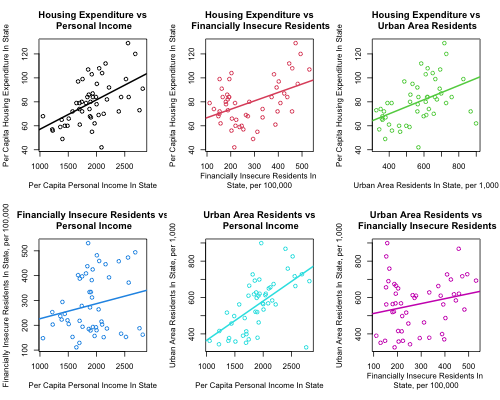
\includegraphics[width=1\textwidth]{political_economy_scatter_plot.png}
\end{figure}
\lstinputlisting[language=R, firstline=99, lastline=140]{PS01_answers_CZ.R}

\vspace{.5cm}
\item
Please plot the relationship between \emph{Y} and \emph{Region}? On average, which region has the highest per capita expenditure on housing assistance?

\begin{verbatim}
	Region 4, the West, has the highest average of per capita expenditure 
	on housing assistance
\end{verbatim}
\vspace{.5cm}
\newpage
\begin{figure}[h!]\centering
	\caption{\footnotesize Housing Expenditure (Per Capita) by Region}
	\label{fig:plot_2}
	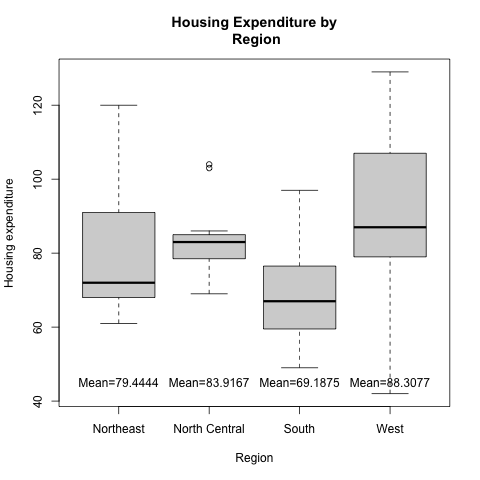
\includegraphics[width=.75\textwidth]{housing_expenditure_region__scatter_plot.png}
\end{figure}
\lstinputlisting[language=R, firstline=146, lastline=165]{PS01_answers_CZ.R}
\vspace{1cm}
\item
Please plot the relationship between \emph{Y} and \emph{X1}? Describe this graph and the relationship. Reproduce the above graph including one more variable \emph{Region} and display different regions with different types of symbols and colors.

\begin{figure}[h!]\centering
	\caption{\footnotesize Figure 3.}
	\label{fig:plot_3}
	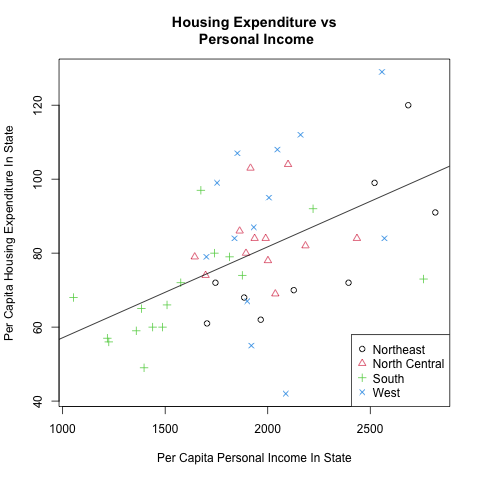
\includegraphics[width=.75\textwidth]{housing_expenditure_personal_income_scatter_plot.png}
\end{figure}
\begin{verbatim}
	The scatterplot of Y (Housing expenditure, per capita in state) vs X1 
	(Personal income, per capita in state), shows a moderate positive 
	linear relationship. As per capita personal income (in state) increases, 
	per capita housing expenditure (in state) tends to increase. Region 4, the 
	West, has the most spread, and region 2 (North Central) has the least 
	spread in terms of housing expenditure. The North Central region is 
	clustered in the middle of the data, the South towards the lower end. The
	South (Region 3) region appears to have a strong positive relationship 
	between	housing expenditure and personal income (per capita). The Northeast
	region (region 1) also appears to have a stroing positive relationship between 
	Y and X1. The North Central region (Region 2) and the West (Region 4) appear 
	to have nonlinear relationships between per capita housing expenditure and 
	per capita personal income, with weak to negligible correlation. 
	
\end{verbatim}

\lstinputlisting[language=R, firstline=169, lastline=178]{PS01_answers_CZ.R}



\end{itemize}


\end{document}
